\subsubsection{Trabajando con matrices}\label{workingwithmatrixes}
Para facilitar la explicación a partir de este punto, se procede a explicar distintas partes de la red y su notación matemática con alguna simplificación.
\newline

Se parte de la siguiente definición de red neuronal:

\begin{figure}[H]
    \centering
    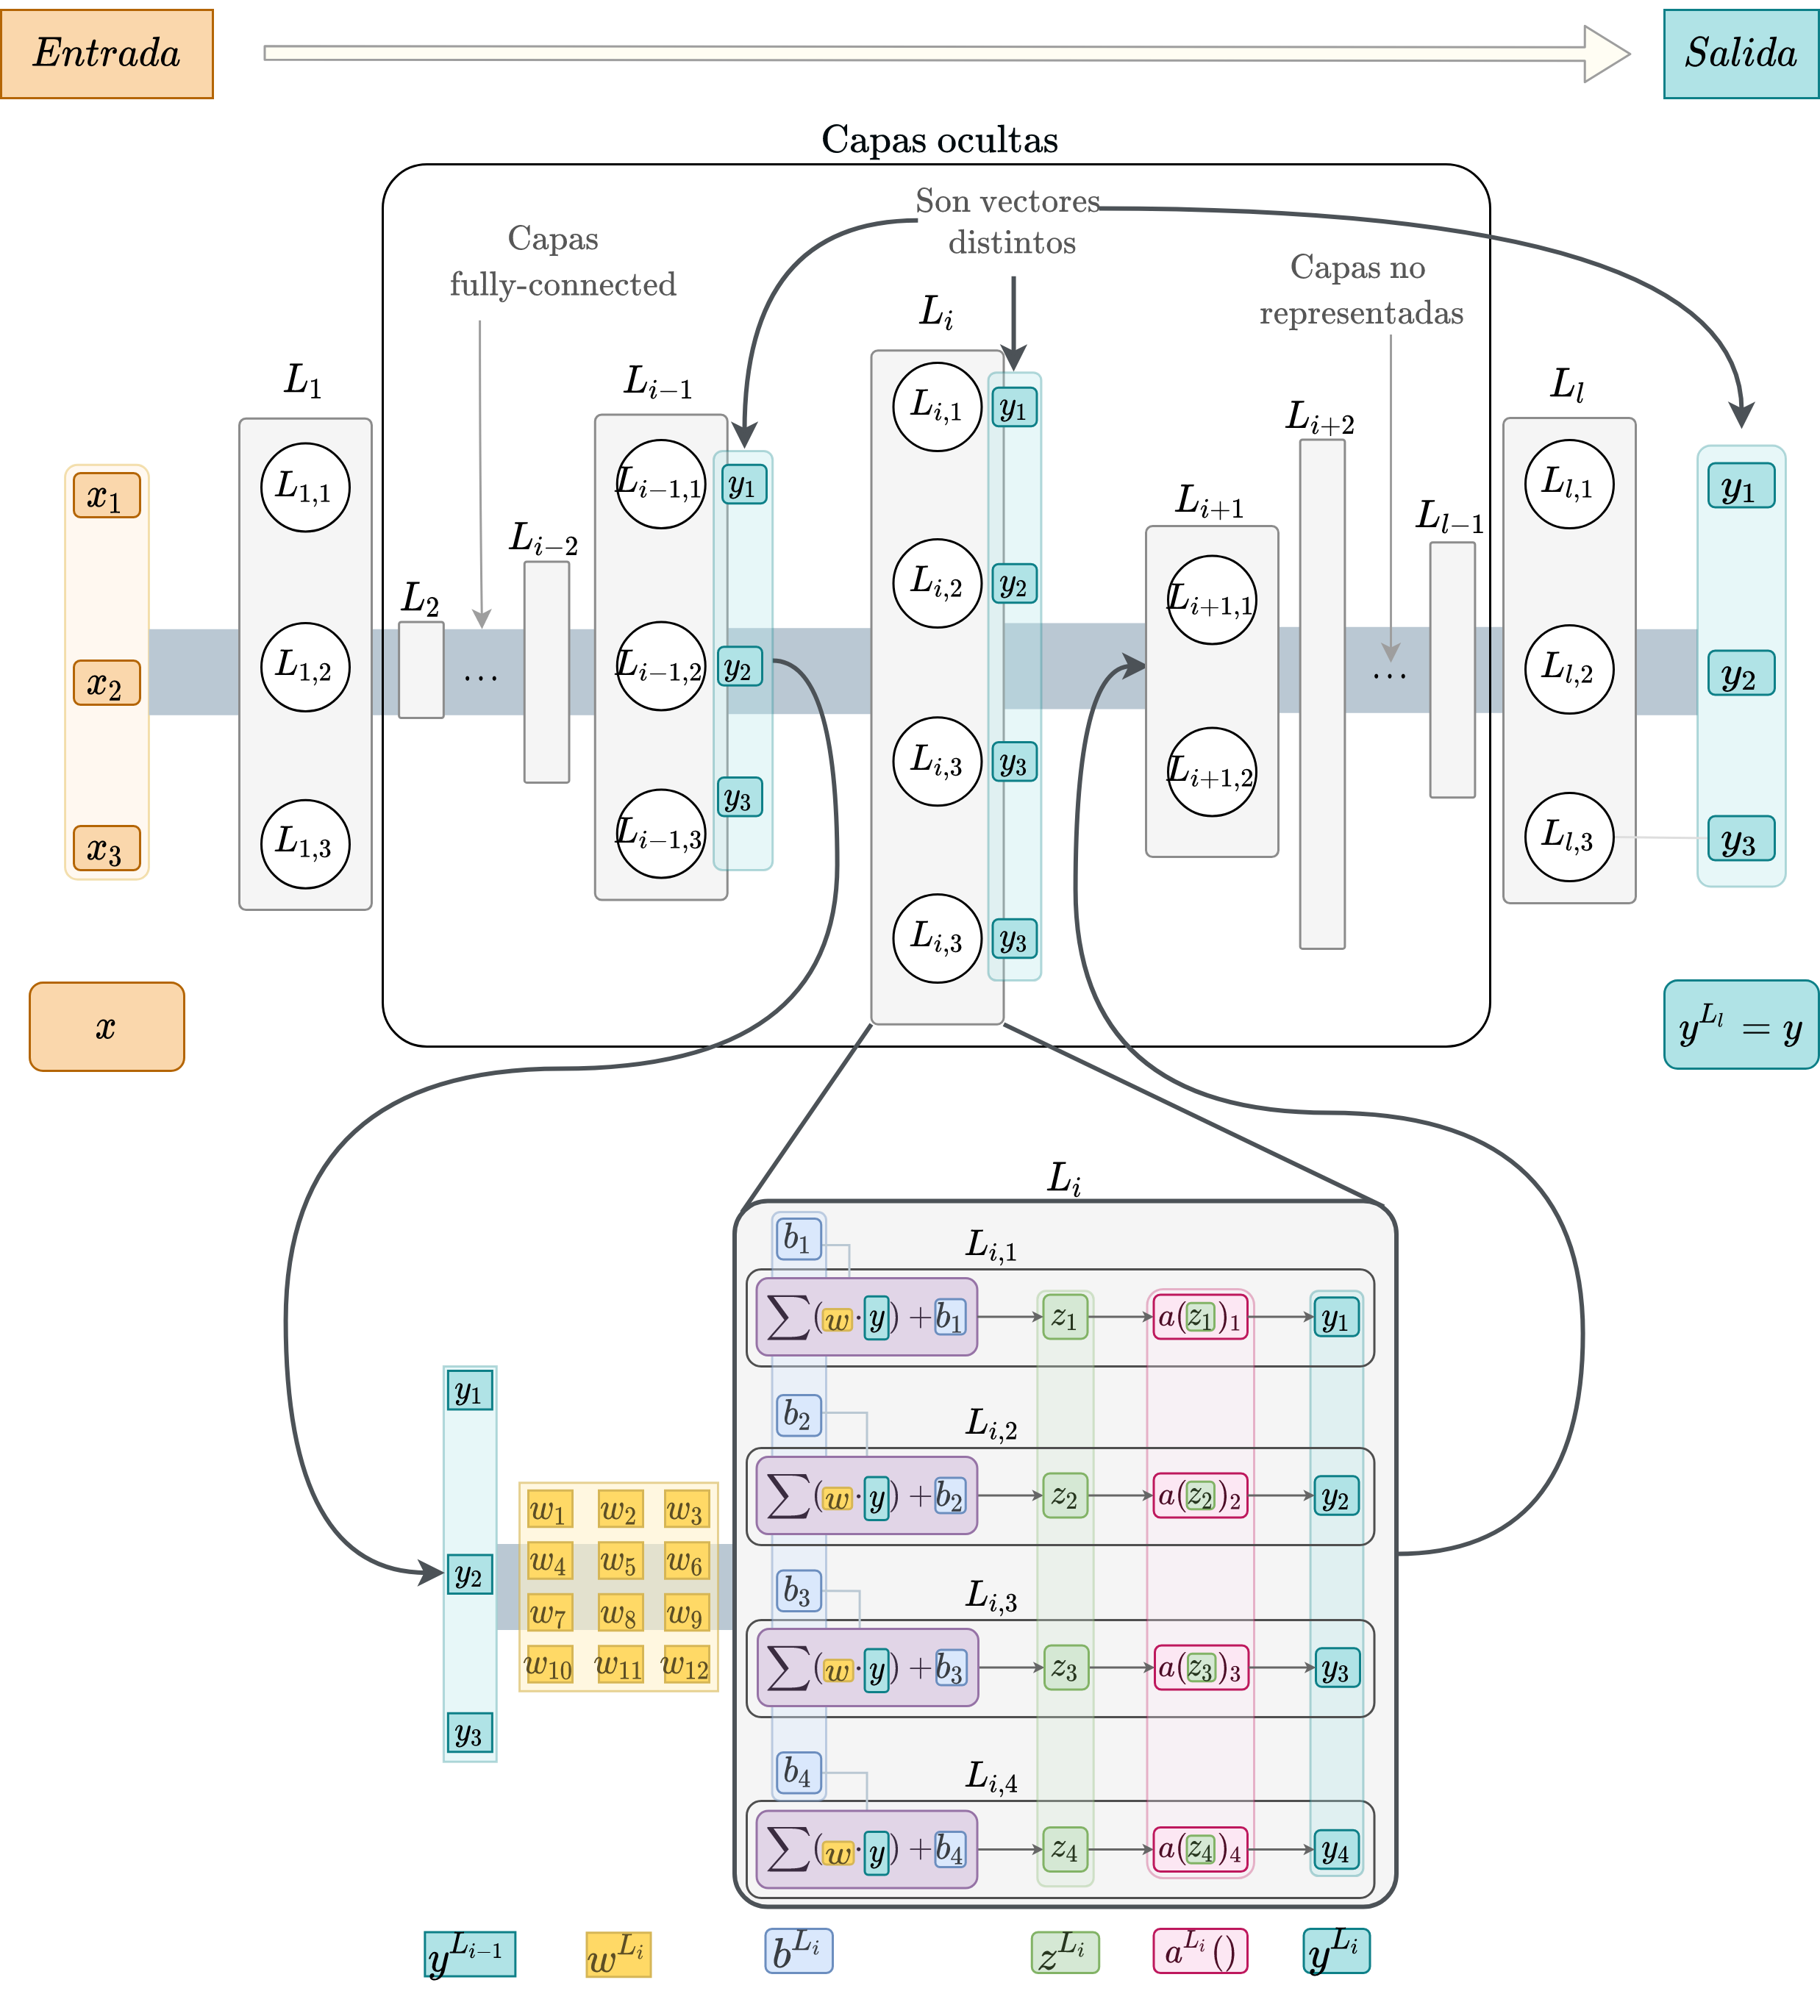
\includegraphics[width=16cm]{images/state-of-art/matrixes/layer_activation_representation.png}
    \caption{Red neuronal}
    \label{fig:basic_network51}
\end{figure}

La red representada necesita tres valores de entrada que devuelve un único valor, así el modelo será entrenado para que, dado un vector de tres elementos, el modelo otros tres elementos. El valor que devuelva el modelo será igual al valor $y$, calculado en la última capa:

\begin{equation}
    \begin{split}
    y = a^{L_3}(z_3) &= w_3 \cdot a^{L_2}(z_2) + b_3 \\ 
    \text{donde}~L_i &= \text{Última capa}  \\
  ~w_j &= \text{Pesos en la última capa } \\ 
  ~b_k &= \text{\textit{Biases} en la última capa} \\
  ~a^{L_{u}}(z_{u}) &= \text{Resultado de la función de activación de la capa } L_{u} \text{ sobre el vector } z_u \\
  ~a^{L_2}(z_2) &= \text{Vector con los valores de la salida de penúltima capa}
  \end{split}
  \label{eqn:layer3}
\end{equation}


El número de elementos de $z_{l-1}$ será el mismo número de neuronas que haya en la capa $L__{l-1}$. Esto ocurre $\forall z_i$. El vector $z__{l-1}$ es calculado en la capa $L__{l-1}$ de la siguiente forma:
\begin{equation}
    z_{L_{l-1}} = w_{L_{l-1}} \cdot a^{L_{l-2}}(z_{L_{l-2}}) + b_{L_{l-1}}
  \label{eqn:layer2}
\end{equation}

Este proceso se repetirá hasta que $z_1$ sea calculado:
\begin{equation}
    \begin{split}
    z_1 &= w_1 \cdot x + b_1 \\
    \text{donde}~x &= \text{Vector de entrada}
  \end{split}
  \label{eqn:layer1}
\end{equation}

Para hacer referencia a una capa de la red se usará $L_i$, siendo $i$ el índice de la capa ($i=1$ para la primera capa, $i=2$ para la segunda capa...). Para hacer referencia a la última capa, se usará $L_l$, la penúltima será $L_{l-1}$ y así sucesivamente. Se puede añadir un segundo índice para hacer referencia a una neurona tal que $L_{i, j}$ y al igual que el índice de capa, si $j=1$, hará referencia a la primera neurona de la capa, si $j=2$, hará referencia a la segunda neurona de la capa y así respectivamente. A modo de ejemplo la tercera neurona de la segunda capa será referenciada como $L_{2, 3}$ o $L_{l-1, 3}$.
\newline

El vector $w$ y valor $b$ de $L_{2, 3}$ serán referenciados tal que $w^{L_{2,3}}$ y $b^{L_{2,3}}$ respectivamente. Si se quiere hacer referencia a un valor del vector $w$ en concreto se usará un tercer índice tal que $w^{L_{i,j}}_k$. Por ejemplo, $w^{L_{2,3}}_1$ hará referencia al primer peso de la tercera neurona de la segunda capa.
\newline

Sabiendo esta nueva notación, a partir de este punto se simplificarán las ecuaciones. Por ello, los parámetros de una neurona vendrán en un único vector añadiendo el valor $b$ al vector ya existente $w$. Todos los vectores se agruparán formando una matriz $W$, donde cada fila será el vector asociado a una neurona. Es decir, los parámetros de una capa $L_i$ vendrá dado como una matriz a la que se hará referencia como $W$. 

\begin{equation}
\centering
    \begin{split}
    W^{L_i} &= \begin{pmatrix}
  b^{L_{i,1}} & w^{L_{i, 1}}_1 & w^{L_{i, 1}}_2 & \cdots & w^{L_{i, 1}}_n \\
  b^{L_{i,2}} & w^{L_{i, 2}}_1 & w^{L_{i, 2}}_2 & \cdots & w^{L_{i, 2}}_n \\
  b^{L_{i,3}} & w^{L_{i, 3}}_1 & w^{L_{i, 3}}_2 & \cdots & w^{L_{i, 3}}_n \\
  \vdots & \vdots  & \vdots & & \vdots \\
  b^{L_{i,m}} & w^{L_{i, m}}_1 & w^{L_{i, m}}_2 & \cdots & w^{L_{i, m}}_n
  \end{pmatrix} \\ 
    \text{donde}~i &= \text{Índice de la capa en la red} \\
  ~n &= \text{Número de neuronas en }L_{i-1}\text{ o longitud de vector de entrada si } i=1 \\
  ~m &= \text{Número de neuronas en la capa } L_i
  \end{split}
  \label{examplenn51}
\end{equation}

Como ejemplo, la matriz $W^{L-1}$ de la red neuronal definida en la figura \ref{fig:basic_network51} sería la siguiente:

\begin{equation}
  W^{L_{l-1}} = W^{L_2} = \begin{pmatrix}
  b_1 & w_1 & w_2 & w_3 \\
  b_2 & w_4 & w_5 & w_6 \\ 
  b_3 & w_7 & w_8 & w_9 \\ 
  b_4 & w_{10} & w_{11} & w_{12}
  \end{pmatrix} 
  \label{eqn:matrixlayer}
\end{equation}



Usando el ejemplo de la figura \ref{fig:xorgatenetwork}, donde se usan valores específicos para $w$ y $b$, las matrices de cada capa con los parámetros quedarían tal que:

\begin{equation}
  W^{L_1} = \begin{pmatrix}
  0 & 1 & 1 \\ 
  -1 & 1 & 1
  \end{pmatrix}
\end{equation}

\begin{equation}
  W^{L_2} = \begin{pmatrix}
  -2 & 3 & -2
  \end{pmatrix}
\end{equation}

Con esta nueva notación en una sola matriz se recoge los parámetros que necesita calcular la regresión. De hecho, esta matriz es los que el modelo tendrá que "aprender" para obtener mejores resultados. Esto se verá más en detalle en la sección \ref{training}.
\newline

En la ecuación \ref{eqn:activationfunctionbasic} se calculaba el valor con la función $a()$ de la neurona. A partir de este punto, una función de activación recibirá un vector con los valores $z$ de cada neurona y por tanto esta función $a()$ también devolverá un vector del mismo tamaño. En la primera capa de la red, este vector será calculado tal que:
\begin{equation}
  y_1 = a^{L_1}(z) = a(W^{L_1}x)
  \label{eqn:activationmatrixwrong}
\end{equation}

Pero al definir la matriz $W$ de esta forma, el producto $W^{L_1}x$ es imposible de calcular. Esto se puede demostrar usando el ejemplo de la figura \ref{examplenn51}. La dimensión de $W^{L_1}$ es $(3 \times 6)$. Sin embargo, el vector $x$ con el que se va a multiplicar tiene una dimensión $(1 \times 5)$. Para solucionar este problema, se añadirá un $1$ al vector $x$, vector conocido como $x'$ y se realizará la transpuesta de dicho vector. De esta forma se podrá multiplicar la matriz $W$ con dimensión $3\times6$ con un vector de dimensión $6\times1$.

\begin{equation}
\centering
    \begin{split}
  a^L_1(z) &= a(W^{L_2}x') \\
    \text{donde}~x' &= [[1] \oplus x]^T = [1, x_1, x_2, ... x_n]^T \\
    n &= \text{Tamaño del vector } x \\
    A \oplus B &: \text{Concatenación de vectores } A \text{ y } B
  \end{split}
  \label{eqn:newactivationsimple}
\end{equation}

El resto de las capas no tiene este problema. El vector obtenido en la anterior capa ya cumple con las condiciones necesarias para poder realizar el productor de una matriz por un vector. El vector $a^{L_2}(z)$ usará la misma ecuación que \ref{eqn:activationmatrixwrong}, pero la variable $x$ será el vector $y$ calculado en la anterior capa:
\begin{equation}
  a^{L_2}(z) = a(W^{L_2} \cdot a(W^{L_1}x'))
\end{equation}

Se realizará este proceso hasta llegar a la última capa de la red. Se puede leer más información en la sección \ref{feedforward}.
\newline


Actualizando también las ecuaciones \ref{eqn:layer3}, \ref{eqn:layer2} y \ref{eqn:layer1}:
\begin{equation}
    y = a^{L_3}(z_3) = W^{L_3} \cdot a^{L_2}(z_2) 
\end{equation}
\begin{equation}
    z_2 = W^{L_2} \cdot a^{L_1}(z_1)
\end{equation}
\begin{equation}
    z_1 = W^{L_1} \cdot x'
\end{equation}

Agrupando todas las ecuaciones en una sola, el valor de $y$ en una red neuronal con tres capas viene dado por:
\begin{equation}
    y = a(W^{L_3} \cdot (a(W^{L_2} \cdot (a(W^{L_1} \cdot x')^{L_1}))^{L_2}))^{L_3}
    \label{eqn:feedforwardexample}
\end{equation}

Esta ecuación es la que resuelve el modelo para poder obtener el valor $y$ y es lo que se conoce como algoritmo de \textit{forward-pass}.
\newline